
\documentclass[a4paper]{article}

%\usepackage[pages=all, color=black, position={current page.south}, placement=bottom, scale=1, opacity=1, vshift=5mm]{background}

\usepackage[margin=1in]{geometry} % full-width

% AMS Packages
\usepackage{amsmath}
\usepackage{amsthm}
\usepackage{amssymb}
\usepackage{booktabs}

% Unicode
\usepackage[utf8]{inputenc}
\usepackage{hyperref}
\newcommand{\AL}[1]{{\color{blue}{[Andrew: #1]}}}

\hypersetup{
	unicode,
%	colorlinks,
%	breaklinks,
%	urlcolor=cyan, 
%	linkcolor=blue, 
	pdfauthor={Author One, Author Two, Author Three},
	pdftitle={A simple article template},
	pdfsubject={A simple article template},
	pdfkeywords={article, template, simple},
	pdfproducer={LaTeX},
	pdfcreator={pdflatex}
}

% Vietnamese
%\usepackage{vntex}

% Natbib
%\usepackage[sort&compress,numbers,square]{natbib}
%\bibliographystyle{mplainnat}

% Theorem, Lemma, etc
\theoremstyle{plain}
\newtheorem{theorem}{Theorem}
\newtheorem{corollary}[theorem]{Corollary}
\newtheorem{lemma}[theorem]{Lemma}
\newtheorem{claim}{Claim}[theorem]
\newtheorem{axiom}[theorem]{Axiom}
\newtheorem{conjecture}[theorem]{Conjecture}
\newtheorem{fact}[theorem]{Fact}
\newtheorem{hypothesis}[theorem]{Hypothesis}
\newtheorem{assumption}[theorem]{Assumption}
\newtheorem{proposition}[theorem]{Proposition}
\newtheorem{criterion}[theorem]{Criterion}
\theoremstyle{definition}
\newtheorem{definition}[theorem]{Definition}
\newtheorem{example}[theorem]{Example}
\newtheorem{remark}[theorem]{Remark}
\newtheorem{problem}[theorem]{Problem}
\newtheorem{principle}[theorem]{Principle}

\usepackage{graphicx, color}
\graphicspath{{fig/}}

%\usepackage[linesnumbered,ruled,vlined,commentsnumbered]{algorithm2e} % use algorithm2e for typesetting algorithms
\usepackage{algorithm, algpseudocode} % use algorithm and algorithmicx for typesetting algorithms
\usepackage{mathrsfs} % for \mathscr command

\usepackage{lipsum}

% Author info
\title{CSC2611 Lab: Word embedding and semantic change}
\author{Yuan-Hong Liao$^{1}$}

\date{
	$^1$Computer Science at the University of Toronto \\ \texttt{andrew@cs.toronto.edu}
}

\begin{document}
\maketitle


\noindent All the code is included at https://github.com/andrewliao11/CSC2611-course/tree/main/assignment1

\section{Synchronic word embedding}

\noindent\textbf{Step 3.}
I show the Pearson correlation between human similarities and the similarities from the various computational methods, such as word2vec, word context model, positive pmi model, and latent semantic model, in Tab.~\ref{tab:pearson-human}.
The dictionary size used in word-context model, positive pmi model, and latent semantic model is 5031. For the target pairs containing out-of-dictionary words, I simiply assign zero cosine similarity (neutral).

Both word-context model and word2vec use the surrounding words to represent a word. However, word2vec leverages the expressibility of neural networks and is trained on larger corpus (33B words vs. 1M in Brown corpus).
Besides, the word-context model only considers the relation from the preceding words to current words, providing uni-directional relations. We should consider bidirectional, instead.

\begin{table}[h]
\resizebox{\textwidth}{!}{%
\begin{tabular}{@{}lcclccc@{}}
\toprule
                                        & word2vec                  & word-context model         & Positive PMI model         & LSA (dim=10)              & LSA (dim=100)              & LSA (dim=300)             \\ \midrule
\multicolumn{1}{r}{Pearson Correlation} & \multicolumn{1}{r}{\textbf{0.772}} & \multicolumn{1}{r}{0.1608} & \multicolumn{1}{r}{0.2385} & \multicolumn{1}{r}{0.223} & \multicolumn{1}{r}{0.3587} & \multicolumn{1}{r}{0.297} \\ \bottomrule
\end{tabular}%
}
\caption{Pearson correlation w.r.t. human similarities.}
\label{tab:pearson-human}
\end{table}


\noindent\textbf{Step 4.} I perform the analogy test with word2vec and various computational mehtods. The data is from the Google analogy test set. 
The results are shown in Fig.~\ref{tab:acc}. Similar to the reasons shown in \textbf{step 3}, the superiority of word2vec is due to the more powerful neural networks and the larger datasets
Also, word2vec considers a larger window size (5), potentially connects words with more abstract relations, such as capital-countries.


\begin{table}[h]
\resizebox{\textwidth}{!}{%
\begin{tabular}{@{}rrrrrr@{}}
\toprule
\multicolumn{1}{l}{} & \multicolumn{1}{c}{Random} & \multicolumn{1}{c}{word2vec} & \multicolumn{1}{c}{word-context model} & \multicolumn{1}{c}{Positive PMI model} & \multicolumn{1}{c}{LSA (dim=300)} \\ \midrule
Top1 Acc.             & 0.055                      & \textbf{0.961}               & 0.367                                  & 0.482                                  & 0.502                             \\ \midrule
Top5 Acc.             & 0.316                      & \textbf{0.999}               & 0.715                                  & 0.796                                  & 0.819                             \\ \bottomrule
\end{tabular}%
}
\caption{Analogy Test results.}
\label{tab:acc}
\end{table}


\noindent\textbf{Step 5.} To make the word-context model better at capturing word similarities, I leverages the bi-directional relations in the corpus and increase the context size to 5 (from 1). In Tab.~\ref{}, I show the resulting performances in word-context model, positive pmi model, and LSA model.

\section{Diachronic word embedding}

\noindent\textbf{Step 2.} Given a set of word embeddings, we need to measure the degree of semantic change for individual words. 
We compare the differences between two embeddings from different time periods $D(e_1, e_2)$ and use it to determine the degree of semantic change.
Here, we have three choice: \textit{i)} l1 norm: $D(e_1, e_2) = |e_1 - e_2|_1$, \textit{ii)} l-$\infty$ norm: $D(e_1, e_2) = |e_1 - e_2|_\infty$, and \textit{iii)} negative cosine similarity: $D(e_1, e_2) = \frac{-e_1 e_2^\top}{|e_1|_2 |e_2|_2}$.
We show the results in Tab.~\ref{tab:semantic_change_top20} and Tab.~\ref{tab:semantic_change_bot20}.
We show the Pearson correlation between three different criterions in Tab.~\ref{tab:change_pearson}


\begin{table}[h]
\resizebox{\textwidth}{!}{%
\begin{tabular}{@{}rl@{}}
\toprule
                             & \multicolumn{1}{c}{Top 20 most changing words}                                                                                                                                        \\ \midrule
l1-norm                      & objectives, programs, computer, radio, approach, sector, goals, van, media, patterns, shri, impact, challenge, perspective, film, berkeley, file, mcgraw, therapy, project       \\ \midrule
l-$\infty$ norm & computer, ball, wiley, storm, coat, sex, answers, shift, signal, strain, survival, components, accounts, others, currency, fortune, means, richard, assessment, energy           \\ \midrule
negative cosine              & programs, objectives, computer, radio, sector, goals, approach, van, shri, media, impact, perspective, patterns, berkeley, shift, film, assessment, stanford, challenge, therapy \\ \bottomrule
\end{tabular}%
}
\caption{Top 20 most changing by different criterions}
\label{tab:semantic_change_top20}
\end{table}

\begin{table}[h]
\resizebox{\textwidth}{!}{%
\begin{tabular}{@{}rl@{}}
\toprule
                             & \multicolumn{1}{c}{Top 20 least changing words}                                                                                                                                            \\ \midrule
l1-norm                      & april, june, november, century, years, october, february, september, feet, months, door, god, disease, payment, increase, daughter, water, evening, week, mother                     \\ \midrule
l-\textbackslash{}infty norm & april, february, evidence, june, november, surface, officials, nerve, brother, voice, provisions, husband, evening, coast, january, officers, favour, parties, september, difference \\ \midrule
negative cosine              & april, june, november, february, years, october, increase, january, century, months, daughter, december, god, september, feet, week, evening, door, payment, miles                   \\ \bottomrule
\end{tabular}%
}
\caption{Top 20 least changing by different criterions}
\label{tab:semantic_change_bot20}
\end{table}


\begin{table}[h]
\centering
\resizebox{0.5\textwidth}{!}{%
\begin{tabular}{@{}rrrr@{}}
\toprule
                & \multicolumn{1}{c}{l1-norm} & \multicolumn{1}{l}{l-$\infty$ norm} & \multicolumn{1}{l}{negative cosine} \\ \midrule
l1-norm         & 1.                          & 0.0996                              & 0.1338                              \\ \midrule
l-$\infty$ norm & 0.0996                      & 1.                                  & 0.0722                              \\ \midrule
negative cosine & 0.1338                      & 0.0722                              & 1.                                  \\ \bottomrule
\end{tabular}%
}
\caption{Pearson correlation between different criterions.}
\label{tab:change_pearson}
\end{table}

\noindent\textbf{Step 3.} To evaluate the accuracy of the proposed methods in Step 2, we need to first identify what the ground truths are.
To this end, we need to incorporate our prior knowledge in word semantics. 
\textit{i)} semantics of number do not change, e.g., hundreds, thousands, millions.
\textit{ii)} semantics of date do not change, e.g., january, feburary, april.
In total, I list out 13 stable words: hundreds, thousands, millions, january, february, april, june, july, august, september, october, november, december.
I report the average rank of the stable words for each criterions in Tab.~\ref{tab:avg_rank} (the lower the better).

\begin{table}[h]
\centering
\resizebox{0.5\textwidth}{!}{%
\begin{tabular}{@{}rcll@{}}
\toprule
          & l1-norm                     & l-$\infty$ norm              & negative cosine             \\ \midrule
Avg. Rank $\downarrow$ & \multicolumn{1}{r}{986.692} & \multicolumn{1}{r}{1196.462} & \multicolumn{1}{r}{792.154} \\ \bottomrule
\end{tabular}%
}
\caption{The average rank of stable words (the lower the better).}
\label{tab:avg_rank}
\end{table}

\noindent\textbf{Step 4.} From the analysis in Step 2 and 3, we choose to use the negative cosine similarity to determine the degree of semantic changes. 
I implement a detecting algorithm that report semantic change whenever the negative cosin values drop over 0.2.
I show the results in Fig.~\ref{fig:change_time}


\begin{figure}[h]
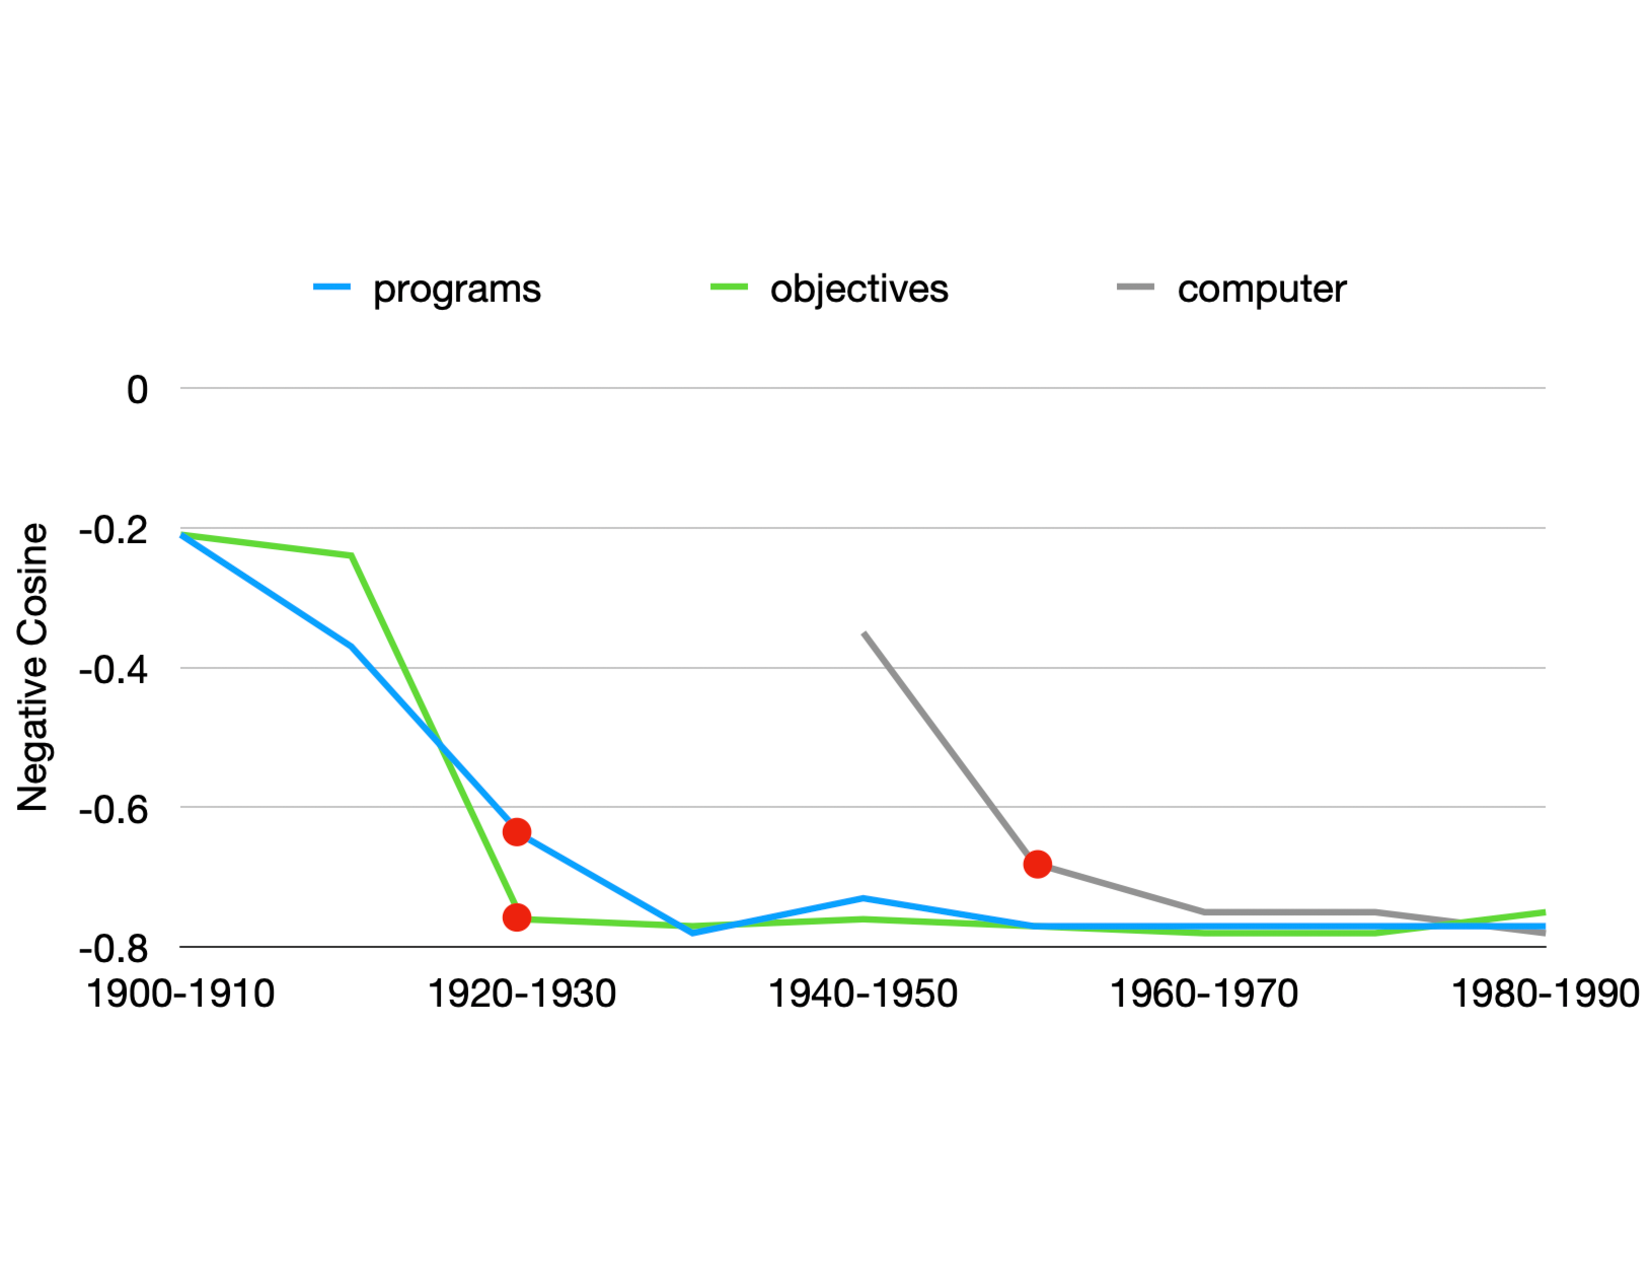
\includegraphics[width=8cm]{change.pdf}
\centering
\caption{The semantic changes happens when the negative cosine values drop a lot.}
\label{fig:change_time}
\end{figure}

\end{document}